% answers.tex —— 2020 年·全国Ⅰ卷·文科 · 参考答案与详细解析片段
% 由 tools/generate_projects.py 依来源总账自 2020/2020_数学真题_文_试题.md + 2020/2020_数学真题_文_解析正文.md + 2020/2020_数学真题_文_答案要点.md 生成，勿手改（改源 MD 后重跑）


\begin{gknotice}
\textbf{解析归属}：本文档全部解析由本库编写者根据试题独立推导，\textbf{非官方标准答案}。若与官方发布版本不一致，以官方为准。

\textbf{与理科卷重合的 8 题}（第 3、5、7、12、13、21、22、23 题）在此给出结论与要点，完整推导见理科卷含解析，避免重复。
\end{gknotice}

\par\medskip

\gkpart{一、选择题（每小题 5 分，共 60 分）}

\begin{answer}
\gksolhead{1}{}

\textbf{题目}：

已知集合 $A=\left\{x\mid x^{2}-3x-4<0\right\}$，$B=\{-4,1,3,5\}$，则 $A\cap B=$（　　）

\begin{gkopts}(4)
\task A．$\{-4,1\}$
\task B．$\{1,5\}$
\task C．$\{3,5\}$
\task D．$\{1,3\}$
\end{gkopts}

\textbf{解析}

因式分解求 $A$：
\[x^{2}-3x-4=(x-4)(x+1)<0\ \Longrightarrow\ -1<x<4\]

逐个检验 $B$ 的元素是否落在 $(-1,4)$ 内：

\begin{center}
\begin{tabular}{ccccc}
\toprule
元素 & $-4$ & $1$ & $3$ & $5$ \\
\midrule
是否满足 &  &  &  &  \\
\bottomrule
\end{tabular}
\end{center}

\[A\cap B=\{1,\ 3\}\]

\gkanswer{答案：D（$\{1,3\}$）}

\par\medskip

\end{answer}
\begin{answer}
\gksolhead{2}{}

\textbf{题目}：

若 $z=1+2\mathrm i+\mathrm i^{3}$，则 $|z|=$（　　）

\begin{gkopts}(4)
\task A．$0$
\task B．$1$
\task C．$\sqrt2$
\task D．$2$
\end{gkopts}

\textbf{解析}

\textbf{关键：先化简 $\mathrm i^{3}$。}

$\mathrm i$ 的幂\textbf{四个一循环}：
\[\mathrm i^{1}=\mathrm i,\quad \mathrm i^{2}=-1,\quad \mathrm i^{3}=-\mathrm i,\quad \mathrm i^{4}=1\]

故
\[z=1+2\mathrm i+(-\mathrm i)=1+\mathrm i\]

\[|z|=\sqrt{1^{2}+1^{2}}=\sqrt2\]

\begin{gktip}
\textbf{易错}：把 $\mathrm i^{3}$ 当成 $\mathrm i$（漏了负号），会得到 $z=1+3\mathrm i$，$|z|=\sqrt{10}$，不在选项中——\textbf{若算出的答案不在选项里，往往就是 $\mathrm i$ 的幂算错了}。
\end{gktip}

\gkanswer{答案：C（$\sqrt2$）}

\par\medskip

\end{answer}
\begin{answer}
\gksolhead{3}{}

\textbf{题目}：

埃及胡夫金字塔是古代世界建筑奇迹之一，它的形状可视为一个正四棱锥，以该四棱锥的高为边长的正方形面积等于该四棱锥一个侧面三角形的面积，则其侧面三角形底边上的高与底面正方形的边长的比值为（　　）

\begin{gkopts}(2)
\task A．$\dfrac{\sqrt5-1}4$
\task B．$\dfrac{\sqrt5-1}2$
\task C．$\dfrac{\sqrt5+1}4$
\task D．$\dfrac{\sqrt5+1}2$
\end{gkopts}

\textbf{解析}

\textbf{解析要点}

设底面边长 $2a$、高 $h$、侧面三角形底边上的高（斜高）$m$：
\[m^{2}=h^{2}+a^{2}\qquad\text{（\text{直角三角形关系}）}\]
\[h^{2}=\frac12\times2a\times m=am\qquad\text{（\text{题目条件}）}\]

联立消 $h$：
\[m^{2}=am+a^{2}\ \Longrightarrow\ \left(\frac ma\right)^{2}-\frac ma-1=0\ \Longrightarrow\ \frac ma=\frac{1+\sqrt5}2\]

所求为斜高与\textbf{底面边长}（$=2a$）之比：
\[\frac m{2a}=\frac{\sqrt5+1}4\]

\gkanswer{答案：C（$\dfrac{\sqrt5+1}4$）}

\par\medskip

\end{answer}
\begin{answer}
\gksolhead{4}{}

\textbf{题目}：

设 $O$ 为正方形 $ABCD$ 的中心，在 $O$，$A$，$B$，$C$，$D$ 中任取 $3$ 点，则取到的 $3$ 点共线的概率为（　　）

\begin{gkopts}(4)
\task A．$\dfrac15$
\task B．$\dfrac25$
\task C．$\dfrac12$
\task D．$\dfrac45$
\end{gkopts}

\textbf{解析}

\textbf{第一步，总的取法数。}

从 $5$ 个点中任取 $3$ 个：
\[C_5^{3}=\frac{5\times4\times3}{3\times2\times1}=10\]

\textbf{第二步，找出共线的三点组（本题的全部内容）。}

正方形的中心 $O$ 位于\textbf{两条对角线的交点}，因此：
\begin{itemize}
\item $A$、$O$、$C$ 三点在对角线 $AC$ 上，\textbf{共线} 
\item $B$、$O$、$D$ 三点在对角线 $BD$ 上，\textbf{共线} 
\end{itemize}

\textbf{其它组合都不共线}：
\begin{itemize}
\item 任取三个顶点（如 $A$、$B$、$C$）：构成直角三角形，不共线
\item 含 $O$ 但两个顶点相邻（如 $A$、$O$、$B$）：$O$ 不在边 $AB$ 上，不共线
\end{itemize}

故共线的三点组恰有 $2$ 组。

\textbf{第三步，求概率。}
\[P=\frac2{10}=\frac15\]

\begin{gktip}
\textbf{方法总结}：这类"几何构型 + 古典概型"的题，关键是\textbf{穷举时按结构分类}（本题按"是否含中心 $O$"、"两个顶点是相邻还是相对"分类），避免漏数或重数。
\end{gktip}

\gkanswer{答案：A（$\dfrac15$）}

\par\medskip

\end{answer}
\begin{answer}
\gksolhead{5}{}

\textbf{题目}：

某校一个课外学习小组为研究某作物种子的发芽率 $y$ 和温度 $x$（单位：$^\circ\mathrm C$）的关系，在 $20$ 个不同的温度条件下进行种子发芽实验，得到下面的散点图：

\begin{center}% 2020 全国Ⅰ卷 理5：发芽率-温度散点图（对数饱和形态，数据点按原图形态示意布点）
\begin{tikzpicture}
\begin{axis}[width=8.8cm, height=5cm, font=\small,
  xlabel={温度$/^{\circ}\mathrm{C}$}, ylabel={发芽率},
  xlabel style={at={(1,0)}, anchor=north west},
  ylabel style={at={(0,1)}, anchor=south, rotate=-90},
  xmin=0, xmax=44, ymin=0, ymax=1.08,
  xtick={0,10,20,30,40},
  ytick={0.2,0.4,0.6,0.8,1.0},
  yticklabels={$20\%$,$40\%$,$60\%$,$80\%$,$100\%$},
  axis lines=left, axis line style={-Stealth}]
  \addplot[only marks, mark=square*, mark size=1.3pt] coordinates {
    (10,0.36) (11.5,0.42) (13,0.50) (14.5,0.55) (16,0.58)
    (17.5,0.62) (19,0.64) (20.5,0.68) (22,0.69) (23.5,0.72)
    (25,0.73) (26.5,0.76) (28,0.76) (29.5,0.79) (31,0.80)
    (33,0.82) (35,0.83) (37,0.86) (39,0.86) (40.5,0.88)};
  \addplot[domain=9:41, samples=80, smooth] {0.35*ln(x)-0.45};
\end{axis}
\end{tikzpicture}
\end{center}

由此散点图，在 $10\ ^\circ\mathrm C$ 至 $40\ ^\circ\mathrm C$ 之间，下面四个回归方程类型中最适宜作为发芽率 $y$ 和温度 $x$ 的回归方程类型的是（　　）

\begin{gkopts}(2)
\task A．$y=a+bx$
\task B．$y=a+bx^{2}$
\task C．$y=a+b\mathrm e^{x}$
\task D．$y=a+b\ln x$
\end{gkopts}

\textbf{解析}

\textbf{解析要点}

散点呈现"低温段快速上升、高温段趋于平缓"的\textbf{饱和型增长}。四个模型中只有对数型 $y=a+b\ln x$ 具有"增长逐渐放缓"的特征。

\gkanswer{答案：D（对数型）}

\par\medskip

\end{answer}
\begin{answer}
\gksolhead{6}{}

\textbf{题目}：

已知圆 $x^{2}+y^{2}-6x=0$，过点 $(1,2)$ 的直线被该圆所截得的弦的长度的最小值为（　　）

\begin{gkopts}(4)
\task A．$1$
\task B．$2$
\task C．$3$
\task D．$4$
\end{gkopts}

\textbf{解析}

\textbf{第一步，化圆的标准方程。}
\[x^{2}-6x+y^{2}=0\ \Longrightarrow\ (x-3)^{2}+y^{2}=9\]

圆心 $C(3,0)$，半径 $r=3$。

\textbf{第二步，判断定点与圆的位置关系。}

设 $M(1,2)$：
\[|CM|=\sqrt{(3-1)^{2}+(0-2)^{2}}=\sqrt{4+4}=2\sqrt2\approx2.83\]

因 $2\sqrt2<3=r$，\textbf{点 $M$ 在圆内}，故过 $M$ 的任意直线都与圆相交，必有弦。

\textbf{第三步，用"弦长模型"求最小值。}

设圆心到弦所在直线的距离为 $d$，则
\[\text{\text{弦长}}=2\sqrt{r^{2}-d^{2}}\]

弦长随 $d$ 增大而\textbf{减小}，故弦最短 $\iff$ $d$ 最大。

由于直线必过 $M$，圆心到它的距离 $d\le|CM|=2\sqrt2$，且\textbf{等号成立当且仅当 $CM\perp$ 该直线}。

\textbf{第四步，代入计算。}
\[\text{\text{弦长}}_{\min}=2\sqrt{r^{2}-|CM|^{2}}=2\sqrt{9-8}=2\times1=2\]

\begin{gktip}
\textbf{必背模型}：过\textbf{圆内定点} $M$ 的弦——
\begin{itemize}
\item \textbf{最长弦}：直径（过圆心时 $d=0$），长 $2r$
\item \textbf{最短弦}：垂直于 $CM$ 的那条，长 $2\sqrt{r^{2}-|CM|^{2}}$
\end{itemize}

这两个结论在选填题中可以直接用。
\end{gktip}

\gkanswer{答案：B（$2$）}

\par\medskip

\end{answer}
\begin{answer}
\gksolhead{7}{}

\textbf{题目}：

设函数 $f(x)=\cos\left(\omega x+\dfrac\pi6\right)$ 在 $[-\pi,\pi]$ 的图象大致如下图，则 $f(x)$ 的最小正周期为（　　）

\begin{center}% 2020 全国Ⅰ卷 理7：f(x)=cos(ωx+π/6) 的图象（按答案 T=4π/3，即 ω=3/2 精确绘制）
\begin{tikzpicture}
\begin{axis}[width=8.6cm, height=4.6cm, font=\small,
  axis lines=middle, xlabel={$x$}, ylabel={$y$},
  xmin=-3.6, xmax=3.7, ymin=-1.35, ymax=1.45,
  xtick={-3.14159, -1.39626, 3.14159},
  xticklabels={$-\pi$, $-\frac{4\pi}{9}$, $\pi$},
  ytick=\empty,
  every axis x label/.style={at={(current axis.right of origin)}, anchor=west},
  every axis y label/.style={at={(current axis.above origin)}, anchor=south}]
  \addplot[domain=-3.14159:3.14159, samples=200, thick] {cos(deg(1.5*x + pi/6))};
  \node[below left, font=\small] at (axis cs:0,0) {$O$};
\end{axis}
\end{tikzpicture}
\end{center}

\begin{gkopts}(4)
\task A．$\dfrac{10\pi}9$
\task B．$\dfrac{7\pi}6$
\task C．$\dfrac{4\pi}3$
\task D．$\dfrac{3\pi}2$
\end{gkopts}

\textbf{解析}

\textbf{解析要点}

由图中标注的零点 $x=-\dfrac{4\pi}9$：
\[-\frac{4\pi}9\omega+\frac\pi6=\frac\pi2+k\pi\ \Longrightarrow\ \omega=\frac{-3-9k}4\]

由图象形状（$\omega>0$ 且周期较大）取 $k=-1$，得 $\omega=\dfrac32$，故 $T=\dfrac{2\pi}{3/2}=\dfrac{4\pi}3$。

\gkanswer{答案：C（$\dfrac{4\pi}3$）}

\par\medskip

\end{answer}
\begin{answer}
\gksolhead{8}{}

\textbf{题目}：

设 $a\log_3 4=2$，则 $4^{-a}=$（　　）

\begin{gkopts}(4)
\task A．$\dfrac1{16}$
\task B．$\dfrac19$
\task C．$\dfrac18$
\task D．$\dfrac16$
\end{gkopts}

\textbf{解析}

\textbf{第一步，解出 $a$（保持对数形式，不求小数）。}
\[a=\frac2{\log_3 4}\]

由\textbf{换底公式的倒数关系} $\dfrac1{\log_3 4}=\log_4 3$：
\[a=2\log_4 3=\log_4 3^{2}=\log_4 9\]

\textbf{第二步，代入所求。}

由对数的定义，$a=\log_4 9$ 意味着
\[4^{a}=9\]

故
\[4^{-a}=\frac1{4^{a}}=\frac19\]

\begin{gktip}
\textbf{方法总结}：见到"$\log$ 与指数混合"的题，\textbf{不要试图算出 $a$ 的小数值}，而应把 $a$ 化成"以所求底数为底的对数"（本题化成 $\log_4 9$），然后直接用定义 $4^{\log_4 9}=9$。核心工具是换底公式的两种形式：
\[\log_a b=\frac{\log_c b}{\log_c a},\qquad \log_a b=\frac1{\log_b a}\]
\end{gktip}

\gkanswer{答案：B（$\dfrac19$）}

\par\medskip

\end{answer}
\begin{answer}
\gksolhead{9}{}

\textbf{题目}：

执行下面的程序框图，则输出的 $n=$（　　）

\begin{center}% 2020 全国Ⅰ卷 文9：累加程序框图（输出 n=17）
\begin{tikzpicture}[font=\small, >=Stealth, node distance=7mm,
  box/.style={draw, minimum height=1.9em, inner xsep=7pt},
  term/.style={draw, rounded corners=7pt, minimum height=1.9em, inner xsep=9pt},
  io/.style={draw, trapezium, trapezium left angle=70, trapezium right angle=110,
             minimum height=1.9em, inner xsep=2pt},
  dec/.style={draw, diamond, aspect=2.4, inner sep=1.5pt}]
  \node[term] (start) {开始};
  \node[box, below=of start] (init) {$n=1$，$S=0$};
  \coordinate[below=4mm of init] (merge);
  \node[box, below=2mm of merge] (acc) {$S=S+n$};
  \node[dec, below=of acc] (cond) {$S\le100$};
  \node[box, left=12mm of acc, minimum width=5.2em] (inc) {$n=n+2$};
  \node[io, below=of cond] (out) {输出 $n$};
  \node[term, below=of out] (end) {结束};
  \draw[->] (start) -- (init);
  \draw[->] (init) -- (acc);
  \draw[->] (acc) -- (cond);
  \draw[->] (cond) -- node[right]{否} (out);
  \draw[->] (out) -- (end);
  \draw[->] (cond) -| node[below, pos=0.18]{是} (inc);
  \draw[->] (inc) |- (merge);
\end{tikzpicture}
\end{center}

\begin{gkopts}(4)
\task A．$17$
\task B．$19$
\task C．$21$
\task D．$23$
\end{gkopts}

\begin{gktip}
\textbf{注}：程序框图（算法初步）在现行新课标中已删除，本题仅作历史资料保留。
\end{gktip}

\textbf{解析}

\textbf{第一步，读懂流程。}

由框图，循环体的执行顺序是：
1. $S=S+n$（先累加）
2. 判断 $S\le100$？
\begin{itemize}
\item \textbf{是} → $n=n+2$ → 回到步骤 1
\item \textbf{否} → 输出 $n$，结束
\end{itemize}

\textbf{第二步，逐轮追踪（列表是最稳妥的做法）。}

初始：$n=1$，$S=0$。

\begin{center}
\begin{tabular}{ccccl}
\toprule
轮次 & 累加前 $n$ & $S=S+n$ 后 & $S\le100$？ & 操作 \\
\midrule
1 & $1$ & $1$ & 是 & $n\to3$ \\
2 & $3$ & $4$ & 是 & $n\to5$ \\
3 & $5$ & $9$ & 是 & $n\to7$ \\
4 & $7$ & $16$ & 是 & $n\to9$ \\
5 & $9$ & $25$ & 是 & $n\to11$ \\
6 & $11$ & $36$ & 是 & $n\to13$ \\
7 & $13$ & $49$ & 是 & $n\to15$ \\
8 & $15$ & $64$ & 是 & $n\to17$ \\
9 & $17$ & $81$ & 是 & $n\to19$ \\
10 & $19$ & $100$ & \textbf{是}（$100\le100$） & $n\to21$ \\
11 & $21$ & $121$ & \textbf{否} & 输出 $n=21$ \\
\bottomrule
\end{tabular}
\end{center}

\textbf{第三步，识别规律加速。}

注意 $S$ 的取值恰好是 $1,4,9,16,25,\cdots$，即\textbf{完全平方数}——这是因为"前 $k$ 个正奇数之和等于 $k^{2}$"：
\[1+3+5+\cdots+(2k-1)=k^{2}\]

$S=100=10^{2}$ 对应累加了前 $10$ 个奇数（最后加的是 $19$），此时 $n$ 变为 $21$；再累加得 $121>100$，输出 $n=21$。

\begin{gktip}
\textbf{易错点}：临界判断 $S=100$ 时，条件是 $S\le100$ 而非 $S<100$，故\textbf{仍要继续一轮}。若误判为跳出，会得到 $n=19$（选项 B）——这正是命题人设置的陷阱。

\textbf{注}：程序框图（算法初步）在现行新课标中已删除，本题仅作历史资料。
\end{gktip}

\gkanswer{答案：C（$21$）}

\par\medskip

\end{answer}
\begin{answer}
\gksolhead{10}{}

\textbf{题目}：

设 $\left\{a_n\right\}$ 是等比数列，且 $a_1+a_2+a_3=1$，$a_2+a_3+a_4=2$，则 $a_6+a_7+a_8=$（　　）

\begin{gkopts}(4)
\task A．$12$
\task B．$24$
\task C．$30$
\task D．$32$
\end{gkopts}

\textbf{解析}

\textbf{核心思想：整体看待"三项一组"。}

注意到
\[a_2+a_3+a_4=a_1q+a_2q+a_3q=q\left(a_1+a_2+a_3\right)\]

即\textbf{后一组是前一组的 $q$ 倍}。故
\[q=\frac{a_2+a_3+a_4}{a_1+a_2+a_3}=\frac21=2\]

同理，$a_6+a_7+a_8$ 相对于 $a_1+a_2+a_3$，每个下标\textbf{后移 $5$ 位}，故是它的 $q^{5}$ 倍：
\[a_6+a_7+a_8=q^{5}\left(a_1+a_2+a_3\right)=2^{5}\times1=32\]

\begin{gktip}
\textbf{方法总结}：等比数列题中，\textbf{只要出现"若干连续项之和"，就把它当作一个整体}——整体之间的比值就是 $q$ 的相应次幂。这比先求 $a_1$、$q$ 再逐项计算快得多，而且本题根本不需要知道 $a_1$。
\end{gktip}

\gkanswer{答案：D（$32$）}

\par\medskip

\end{answer}
\begin{answer}
\gksolhead{11}{}

\textbf{题目}：

设 $F_1$，$F_2$ 是双曲线 $C:x^{2}-\dfrac{y^{2}}3=1$ 的两个焦点，$O$ 为坐标原点，点 $P$ 在 $C$ 上且 $|OP|=2$，则 $\triangle PF_1F_2$ 的面积为（　　）

\begin{gkopts}(4)
\task A．$\dfrac72$
\task B．$3$
\task C．$\dfrac52$
\task D．$2$
\end{gkopts}

\textbf{解析}

\textbf{第一步，求出基本量。}
\[a^{2}=1,\quad b^{2}=3,\quad c^{2}=a^{2}+b^{2}=4\ \Longrightarrow\ c=2\]

故 $F_1(-2,0)$、$F_2(2,0)$，$\left|F_1F_2\right|=2c=4$。

\textbf{第二步（本题的题眼）：由 $|OP|=2$ 识别直角。}

注意 $|OP|=2=c$，而 $O$ 是 $F_1F_2$ 的中点、$\left|OF_1\right|=\left|OF_2\right|=c=2$。

这说明 $P$ 到 $F_1F_2$ 中点的距离等于该线段的一半，即 \textbf{$P$ 在以 $F_1F_2$ 为直径的圆上}。

由"直径所对的圆周角是直角"：
\[\angle F_1PF_2=90^\circ\]

\textbf{第三步，联立双曲线定义与勾股定理。}

设 $m=\left|PF_1\right|$、$n=\left|PF_2\right|$。

\begin{itemize}
\item \textbf{双曲线定义}：$|m-n|=2a=2$
\item \textbf{勾股定理}：$m^{2}+n^{2}=\left|F_1F_2\right|^{2}=16$
\end{itemize}

由 $(m-n)^{2}=m^{2}+n^{2}-2mn$：
\[4=16-2mn\ \Longrightarrow\ mn=6\]

\textbf{第四步，求面积。}

直角三角形的面积等于两直角边乘积的一半：
\[S=\frac12mn=\frac12\times6=3\]

\begin{gktip}
\textbf{方法总结}：焦点三角形问题的通用套路是"\textbf{定义式（和或差） + 余弦定理（或勾股）}"联立，通过\textbf{平方}建立起 $mn$ 与已知量的关系，从而求出面积（面积公式 $S=\dfrac12mn\sin\theta$ 只需 $mn$ 的乘积，不需要分别求出 $m$、$n$）。

本题中"$|OP|=c$ ~$\Longrightarrow$~ 直角"这个识别是关键——\textbf{中线等于斜边一半的三角形是直角三角形}。
\end{gktip}

\gkanswer{答案：B（$3$）}

\par\medskip

\end{answer}
\begin{answer}
\gksolhead{12}{}

\textbf{题目}：

已知 $A$，$B$，$C$ 为球 $O$ 的球面上的三个点，$\odot O_1$ 为 $\triangle ABC$ 的外接圆。若 $\odot O_1$ 的面积为 $4\pi$，$AB=BC=AC=OO_1$，则球 $O$ 的表面积为（　　）

\begin{gkopts}(4)
\task A．$64\pi$
\task B．$48\pi$
\task C．$36\pi$
\task D．$32\pi$
\end{gkopts}

\textbf{解析}

\textbf{解析要点}

由 $\odot O_1$ 面积 $4\pi$ 得 $r=2$；等边三角形边长 $=r\sqrt3=2\sqrt3$，故 $OO_1=2\sqrt3$。

由核心公式 $R^{2}=OO_1^{2}+r^{2}=12+4=16$ 得 $R=4$，表面积
\[S=4\pi R^{2}=64\pi\]

\gkanswer{答案：A（$64\pi$）}

\par\medskip

\end{answer}
\gkpart{二、填空题（每小题 5 分，共 20 分）}

\begin{answer}
\gksolhead{13}{}

\textbf{题目}：

若 $x$，$y$ 满足约束条件 $\begin{cases}2x+y-2\le0\\ x-y-1\ge0\\ y+1\ge0\end{cases}$，则 $z=x+7y$ 的最大值为 \gkblank{}．

\textbf{解析}

\textbf{解析要点}

三个顶点为 $(1,0)$、$(0,-1)$、$\left(\dfrac32,-1\right)$，代入目标函数分别得 $1$、$-7$、$-\dfrac{11}2$。

\gkanswer{答案：$1$}

\par\medskip

\end{answer}
\begin{answer}
\gksolhead{14}{}

\textbf{题目}：

设向量 $\boldsymbol a=(1,-1)$，$\boldsymbol b=(m+1,\ 2m-4)$，若 $\boldsymbol a\perp\boldsymbol b$，则 $m=$ \gkblank{}．

\textbf{解析}

垂直 $\iff$ 数量积为零：
\[\boldsymbol a\cdot\boldsymbol b=1\times(m+1)+(-1)\times(2m-4)=0\]

\[m+1-2m+4=0\ \Longrightarrow\ -m+5=0\ \Longrightarrow\ m=5\]

\begin{gktip}
\textbf{提醒}：向量\textbf{垂直}用数量积为零（$x_1x_2+y_1y_2=0$），向量\textbf{平行}用交叉相乘相减为零（$x_1y_2-x_2y_1=0$）。两个判据不能混用。
\end{gktip}

\gkanswer{答案：$5$}

\par\medskip

\end{answer}
\begin{answer}
\gksolhead{15}{}

\textbf{题目}：

曲线 $y=\ln x+x+1$ 的一条切线的斜率为 $2$，则该切线的方程为 \gkblank{}．

\textbf{解析}

\textbf{第一步，由斜率求切点横坐标。}
\[y'=\frac1x+1\]

令 $y'=2$：
\[\frac1x+1=2\ \Longrightarrow\ \frac1x=1\ \Longrightarrow\ x=1\]

\textbf{第二步，求切点纵坐标。}
\[y(1)=\ln1+1+1=0+2=2\]

切点为 $(1,\ 2)$。

\textbf{第三步，写切线方程。}
\[y-2=2(x-1)\ \Longrightarrow\ y=2x\]

\begin{gktip}
\textbf{注}：这条切线恰好过原点，是一个"巧合"，也是命题人让答案简洁的设计。检验：$2\times1=2$  切点确实在切线上。
\end{gktip}

\gkanswer{答案：$y=2x$}

\par\medskip

\end{answer}
\begin{answer}
\gksolhead{16}{}

\textbf{题目}：

数列 $\left\{a_n\right\}$ 满足 $a_{n+2}+(-1)^{n}a_n=3n-1$，前 $16$ 项和为 $540$，则 $a_1=$ \gkblank{}．

\textbf{解析}

\textbf{第一步（关键）：按 $n$ 的奇偶把递推式拆成两个。}

\[(-1)^{n}=\begin{cases}+1,&n\ \text{\text{为偶数}}\\ -1,&n\ \text{\text{为奇数}}\end{cases}\]

故
\[\begin{cases}a_{n+2}+a_n=3n-1,&n\ \text{\text{为偶数}}\quad(\text{\text{相加型}})\\[1mm] a_{n+2}-a_n=3n-1,&n\ \text{\text{为奇数}}\quad(\text{\text{相减型}})\end{cases}\]

\textbf{这两种类型的处理方式完全不同}：相加型可以直接得到"两项之和"，相减型需要逐项累加。

\textbf{第二步，处理偶数项（相加型，直接求和）。}

取 $n=2,6,10,14$（\textbf{注意跳着取，使每两项配成一组、不重不漏}）：
\[a_4+a_2=3\times2-1=5\]
\[a_8+a_6=3\times6-1=17\]
\[a_{12}+a_{10}=3\times10-1=29\]
\[a_{16}+a_{14}=3\times14-1=41\]

\textbf{偶数项之和}：
\[a_2+a_4+\cdots+a_{16}=5+17+29+41=92\]

\textbf{第三步，处理奇数项（相减型，逐项累加）。}

取 $n=1,3,5,\cdots,13$：
\[a_3-a_1=2,\quad a_5-a_3=8,\quad a_7-a_5=14,\quad a_9-a_7=20,\]
\[a_{11}-a_9=26,\quad a_{13}-a_{11}=32,\quad a_{15}-a_{13}=38\]

\textbf{逐个累加得到各项}（都用 $a_1$ 表示）：
\[a_3=a_1+2\]
\[a_5=a_3+8=a_1+10\]
\[a_7=a_5+14=a_1+24\]
\[a_9=a_7+20=a_1+44\]
\[a_{11}=a_9+26=a_1+70\]
\[a_{13}=a_{11}+32=a_1+102\]
\[a_{15}=a_{13}+38=a_1+140\]

\textbf{奇数项之和}（共 $8$ 项）：
\[8a_1+(0+2+10+24+44+70+102+140)=8a_1+392\]

\textbf{第四步，联立求 $a_1$。}
\[\underbrace{8a_1+392}_{\text{\text{奇数项}}}+\underbrace{92}_{\text{\text{偶数项}}}=540\]

\[8a_1=540-484=56\ \Longrightarrow\ a_1=7\]

\begin{gktip}
\textbf{方法总结}：含 $(-1)^{n}$ 的递推数列，\textbf{第一步永远是按奇偶拆开}。拆开后要认清两种类型：
\begin{itemize}
\item \textbf{相加型}（$a_{n+2}+a_n=f(n)$）：直接给出两项之和，适合分组求和，\textbf{不必求通项}
\item \textbf{相减型}（$a_{n+2}-a_n=f(n)$）：是等差型递推，需要\textbf{累加}求出各项
\end{itemize}

本题的巧妙之处在于：偶数项用相加型可以直接算出总和（不需要知道任何一项的具体值），而奇数项用相减型只能全部用 $a_1$ 表示——两部分性质不同，恰好让 $a_1$ 成为唯一未知数。
\end{gktip}

\gkanswer{答案：$7$}

\par\medskip

\end{answer}
\gkpart{三、解答题}

\begin{answer}
\gksolhead{17}{12 分}

\textbf{题目}（12 分）：

某厂接受了一项加工业务，加工出来的产品（单位：件）按标准分为 $A$，$B$，$C$，$D$ 四个等级。加工业务约定：对于 $A$ 级品、$B$ 级品、$C$ 级品，厂家每件分别收取加工费 $90$ 元、$50$ 元、$20$ 元；对于 $D$ 级品，厂家每件要赔偿原料损失费 $50$ 元。该厂有甲、乙两个分厂可承接加工业务。甲分厂加工成本费为 $25$ 元/件，乙分厂加工成本费为 $20$ 元/件。厂家为决定由哪个分厂承接加工业务，在两个分厂各试加工了 $100$ 件这种产品，并统计了这些产品的等级，整理如下：

\textbf{甲分厂产品等级的频数分布表}

\begin{center}
\begin{tabular}{ccccc}
\toprule
等级 & $A$ & $B$ & $C$ & $D$ \\
\midrule
频数 & $40$ & $20$ & $20$ & $20$ \\
\bottomrule
\end{tabular}
\end{center}

\textbf{乙分厂产品等级的频数分布表}

\begin{center}
\begin{tabular}{ccccc}
\toprule
等级 & $A$ & $B$ & $C$ & $D$ \\
\midrule
频数 & $28$ & $17$ & $34$ & $21$ \\
\bottomrule
\end{tabular}
\end{center}

  (1) 分别估计甲、乙两分厂加工出来的一件产品为 $A$ 级品的概率；

  (2) 分别求甲、乙两分厂加工出来的 $100$ 件产品的平均利润，以平均利润为依据，厂家应选哪个分厂承接加工业务？

\textbf{解析}

\par\medskip

\textbf{(1) 解}

用\textbf{频率估计概率}：

\textbf{甲分厂}：$100$ 件中 $A$ 级品有 $40$ 件，
\[P_{\text{\text{甲}}}(A)\approx\frac{40}{100}=0.4\]

\textbf{乙分厂}：$100$ 件中 $A$ 级品有 $28$ 件，
\[P_{\text{\text{乙}}}(A)\approx\frac{28}{100}=0.28\]

\par\medskip

\textbf{(2) 解}

\textbf{第一步，算出每个等级的单件利润。}

利润 = 收取的加工费 $-$ 加工成本。注意 $D$ 级品是\textbf{赔偿 $50$ 元}（收入为 $-50$），成本仍要付。

\textbf{甲分厂（成本 $25$ 元/件）}：

\begin{center}
\begin{tabular}{lcccc}
\toprule
等级 & $A$ & $B$ & $C$ & $D$ \\
\midrule
收入 & $90$ & $50$ & $20$ & $-50$ \\
利润 & $90-25=65$ & $50-25=25$ & $20-25=-5$ & $-50-25=-75$ \\
\bottomrule
\end{tabular}
\end{center}

\textbf{乙分厂（成本 $20$ 元/件）}：

\begin{center}
\begin{tabular}{lcccc}
\toprule
等级 & $A$ & $B$ & $C$ & $D$ \\
\midrule
收入 & $90$ & $50$ & $20$ & $-50$ \\
利润 & $70$ & $30$ & $0$ & $-70$ \\
\bottomrule
\end{tabular}
\end{center}

\textbf{第二步，算 $100$ 件的总利润。}

\textbf{甲分厂}：
\[40\times65+20\times25+20\times(-5)+20\times(-75)\]
\[=2600+500-100-1500=1500\ (\text{\text{元}})\]

平均利润：
\[\frac{1500}{100}=15\ (\text{\text{元}/\text{件}})\]

\textbf{乙分厂}：
\[28\times70+17\times30+34\times0+21\times(-70)\]
\[=1960+510+0-1470=1000\ (\text{\text{元}})\]

平均利润：
\[\frac{1000}{100}=10\ (\text{\text{元}/\text{件}})\]

\textbf{第三步，作出决策。}

因
\[15>10\]

\textbf{厂家应选择甲分厂承接加工业务。}

\begin{gktip}
\textbf{易错点}：$D$ 级品的利润容易只写成 $-50$ 而\textbf{漏掉成本}。正确理解是：厂家不但收不到加工费，还要赔偿 $50$ 元，同时分厂的加工成本照付，故利润为 $-50-\text{\text{成本}}$。

\textbf{另一个观察}：乙分厂虽然成本更低（每件省 $5$ 元），但它的 $A$ 级品率低（$28\%$ vs $40\%$）、$C$ 级品率高（$34\%$ vs $20\%$），产品质量的差距远超成本优势。这也是本题的现实意义——\textbf{决策要看综合收益，不能只看成本}。
\end{gktip}

\gkanswer{答案（1）：甲 $0.4$，乙 $0.28$}

\gkanswer{答案（2）：甲平均利润 $15$ 元、乙 $10$ 元，应选甲分厂}

\par\medskip

\end{answer}
\begin{answer}
\gksolhead{18}{12 分}

\textbf{题目}（12 分）：

$\triangle ABC$ 的内角 $A$，$B$，$C$ 的对边分别为 $a$，$b$，$c$。已知 $B=150^\circ$。

  (1) 若 $a=\sqrt3c$，$b=2\sqrt7$，求 $\triangle ABC$ 的面积；

  (2) 若 $\sin A+\sqrt3\sin C=\dfrac{\sqrt2}2$，求 $C$。

\textbf{解析}

\par\medskip

\textbf{(1) 解}

\textbf{用余弦定理}（已知 $B$ 及其对边 $b$，且 $a$、$c$ 有比例关系）：
\[b^{2}=a^{2}+c^{2}-2ac\cos B\]

代入 $a=\sqrt3c$、$b=2\sqrt7$、$\cos150^\circ=-\dfrac{\sqrt3}2$：
\[28=3c^{2}+c^{2}-2\times\sqrt3c\times c\times\left(-\frac{\sqrt3}2\right)\]

\[28=4c^{2}+\sqrt3c^{2}\times\sqrt3=4c^{2}+3c^{2}=7c^{2}\]

\[c^{2}=4\ \Longrightarrow\ c=2,\qquad a=\sqrt3c=2\sqrt3\]

\textbf{求面积}：
\[S=\frac12ac\sin B=\frac12\times2\sqrt3\times2\times\sin150^\circ=\frac12\times4\sqrt3\times\frac12=\sqrt3\]

\textbf{所以 $\triangle ABC$ 的面积为 $\sqrt3$。}

\par\medskip

\textbf{(2) 解}

\textbf{第一步，消元。}

由内角和 $A+B+C=180^\circ$ 与 $B=150^\circ$：
\[A+C=30^\circ\ \Longrightarrow\ A=30^\circ-C\]

（同时得到 $C$ 的取值范围：$0^\circ<C<30^\circ$。）

\textbf{第二步，代入并展开。}
\[\sin A+\sqrt3\sin C=\sin\left(30^\circ-C\right)+\sqrt3\sin C\]

展开第一项：
\[=\underbrace{\sin30^\circ\cos C-\cos30^\circ\sin C}_{\sin(30^\circ-C)}+\sqrt3\sin C\]
\[=\frac12\cos C-\frac{\sqrt3}2\sin C+\sqrt3\sin C\]
\[=\frac12\cos C+\frac{\sqrt3}2\sin C\]

\textbf{第三步（关键）：用辅助角公式合并。}

注意 $\dfrac{\sqrt3}2=\cos30^\circ$、$\dfrac12=\sin30^\circ$：
\[\frac{\sqrt3}2\sin C+\frac12\cos C=\sin C\cos30^\circ+\cos C\sin30^\circ=\sin\left(C+30^\circ\right)\]

\textbf{第四步，解方程。}
\[\sin\left(C+30^\circ\right)=\frac{\sqrt2}2\]

由第一步，$C\in\left(0^\circ,30^\circ\right)$，故
\[C+30^\circ\in\left(30^\circ,\ 60^\circ\right)\]

在这个范围内，$\sin\theta=\dfrac{\sqrt2}2$ 只有一个解：
\[C+30^\circ=45^\circ\ \Longrightarrow\ C=15^\circ\]

\textbf{所以 $C=15^\circ$。}

\begin{gktip}
\textbf{方法总结}：解三角形中含 $\sin A+\lambda\sin C$ 型条件时，标准路线是"\textbf{用内角和消去一个角 → 展开 → 辅助角合并成单个正弦}"。第三步的合并是本题的技术核心：合并后左边成为单一的 $\sin(\cdot)$，方程立刻可解。

\textbf{务必先确定角的范围}（本题 $C+30^\circ\in(30^\circ,60^\circ)$），否则 $\sin\theta=\dfrac{\sqrt2}2$ 会有 $45^\circ$ 与 $135^\circ$ 两个解。
\end{gktip}

\gkanswer{答案（1）：面积 $=\sqrt3$}

\gkanswer{答案（2）：$C=15^\circ$}

\par\medskip

\end{answer}
\begin{answer}
\gksolhead{19}{12 分}

\textbf{题目}（12 分）：

如图，$D$ 为圆锥的顶点，$O$ 是圆锥底面的圆心，$\triangle ABC$ 是底面的内接正三角形，$P$ 为 $DO$ 上一点，$\angle APC=90^\circ$。

\begin{center}% 2020 全国Ⅰ卷 文19：圆锥（顶点 D，圆心 O，△ABC 内接正三角形，P 在 DO 上，∠APC=90°）
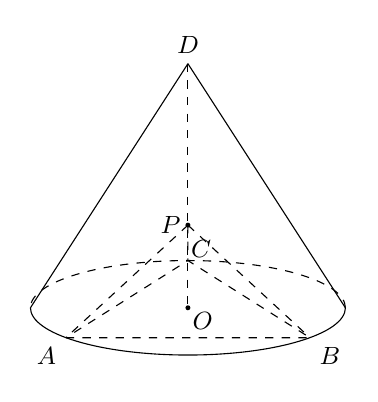
\begin{tikzpicture}[scale=1.0, font=\small]
  \coordinate (D) at (0,3.1);
  \coordinate (O) at (0,0);
  \coordinate (A) at (-1.55,-0.38);
  \coordinate (B) at (1.55,-0.38);
  \coordinate (C) at (0,0.6);
  \coordinate (P) at (0,1.05);
  \draw (-2,0) arc (180:360:2 and 0.6);
  \draw[dashed] (2,0) arc (0:180:2 and 0.6);
  \draw (D) -- (-2,0);
  \draw (D) -- (2,0);
  \draw[dashed] (D) -- (O);
  \draw[dashed] (A) -- (B) -- (C) -- cycle;
  \draw[dashed] (P) -- (A)  (P) -- (B)  (P) -- (C);
  \fill (O) circle (0.9pt);  \fill (P) circle (0.9pt);
  \node[above] at (D) {$D$};
  \node[below left] at (A) {$A$};
  \node[below right] at (B) {$B$};
  \node[above right, inner sep=1pt] at (C) {$C$};
  \node[below right, inner sep=1.5pt] at (O) {$O$};
  \node[left, inner sep=2.5pt] at (P) {$P$};
\end{tikzpicture}
\end{center}

  (1) 证明：平面 $PAB\perp$ 平面 $PAC$；

  (2) 设 $DO=\sqrt2$，圆锥的侧面积为 $\sqrt3\pi$，求三棱锥 $P\text{-}ABC$ 的体积。

\textbf{解析}

  (1) 证明：平面 $PAB\perp$ 平面 $PAC$；(2) 设 $DO=\sqrt2$，圆锥侧面积为 $\sqrt3\pi$，求三棱锥 $P\text{-}ABC$ 的体积。

\par\medskip

\textbf{(1) 证明}

\textbf{第一步，利用对称性。}

$P$ 在圆锥的轴 $DO$ 上，而 $A$、$B$、$C$ 是底面圆上的三个点，且 $\triangle ABC$ 是\textbf{正三角形}（三点关于轴对称分布）。

由于 $PO\perp$ 底面且 $OA=OB=OC$（都是底面半径），故
\[PA=PB=PC=\sqrt{PO^{2}+OA^{2}}\]

\textbf{第二步，由对称性推广已知的直角。}

三条棱 $PA$、$PB$、$PC$ 长度相等，且 $A$、$B$、$C$ 关于轴呈 $120^\circ$ 均匀分布，因此三个角 $\angle APB$、$\angle BPC$、$\angle APC$ \textbf{完全对称、大小相等}。

已知 $\angle APC=90^\circ$，故
\[\angle APB=\angle BPC=\angle APC=90^\circ\]

\textbf{第三步，用线面垂直的判定。}

由 $\angle APB=90^\circ$ 得 $PB\perp PA$；由 $\angle BPC=90^\circ$ 得 $PB\perp PC$。

而 $PA$ 与 $PC$ 是平面 $PAC$ 内的\textbf{两条相交直线}（交于 $P$），由线面垂直的判定定理：
\[PB\perp\text{\text{平面} }PAC\]

\textbf{第四步，用面面垂直的判定。}

$PB\subset$ 平面 $PAB$，而 $PB\perp$ 平面 $PAC$，故
\[\text{\text{平面} }PAB\perp\text{\text{平面} }PAC\qquad\blacksquare\]

\par\medskip

\textbf{(2) 解}

\textbf{第一步，由侧面积求底面半径。}

设底面半径为 $r$，圆锥的高 $DO=\sqrt2$，则母线
\[l=\sqrt{r^{2}+DO^{2}}=\sqrt{r^{2}+2}\]

侧面积公式 $S_{\text{\text{侧}}}=\pi rl$：
\[\pi r\sqrt{r^{2}+2}=\sqrt3\pi\ \Longrightarrow\ r\sqrt{r^{2}+2}=\sqrt3\]

两边平方：
\[r^{2}\left(r^{2}+2\right)=3\ \Longrightarrow\ r^{4}+2r^{2}-3=0\ \Longrightarrow\ \left(r^{2}+3\right)\left(r^{2}-1\right)=0\]

因 $r>0$：
\[r=1\]

\textbf{第二步，求底面正三角形的面积。}

正三角形内接于半径 $r=1$ 的圆，边长
\[AC=r\sqrt3=\sqrt3\]

\[S_{\triangle ABC}=\frac{\sqrt3}4\times\left(\sqrt3\right)^{2}=\frac{3\sqrt3}4\]

\textbf{第三步，由 $\angle APC=90^\circ$ 定出 $P$ 的位置。}

$\triangle APC$ 中 $PA=PC$ 且 $\angle APC=90^\circ$，是\textbf{等腰直角三角形}，斜边 $AC=\sqrt3$：
\[PA=PC=\frac{AC}{\sqrt2}=\frac{\sqrt3}{\sqrt2}=\frac{\sqrt6}2\]

再由 $PA^{2}=PO^{2}+OA^{2}$（$PO\perp$ 底面）：
\[\frac64=PO^{2}+1^{2}\ \Longrightarrow\ PO^{2}=\frac32-1=\frac12\ \Longrightarrow\ PO=\frac{\sqrt2}2\]

\textbf{第四步，求体积。}

三棱锥 $P\text{-}ABC$ 以 $\triangle ABC$ 为底、$PO$ 为高：
\[V=\frac13\times S_{\triangle ABC}\times PO=\frac13\times\frac{3\sqrt3}4\times\frac{\sqrt2}2=\frac{3\sqrt6}{24}=\frac{\sqrt6}8\]

\textbf{所以三棱锥 $P\text{-}ABC$ 的体积为 $\dfrac{\sqrt6}8$。}

\begin{gktip}
\textbf{注意}：题目给的 $DO=\sqrt2$ 只用于\textbf{通过侧面积求出 $r$}，而三棱锥的高是 $PO$（不是 $DO$）——$P$ 的位置由 $\angle APC=90^\circ$ 单独确定。\textbf{读题时务必分清 $D$（圆锥顶点）与 $P$（轴上的点）。}
\end{gktip}

\gkanswer{答案（1）：见解析版}

\gkanswer{答案（2）：$V=\dfrac{\sqrt6}8$}

\par\medskip

\end{answer}
\begin{answer}
\gksolhead{20}{12 分}

\textbf{题目}（12 分）：

已知函数 $f(x)=\mathrm e^{x}-a(x+2)$。

  (1) 当 $a=1$ 时，讨论 $f(x)$ 的单调性；

  (2) 若 $f(x)$ 有两个零点，求 $a$ 的取值范围。

\textbf{解析}

\par\medskip

\textbf{(1) 解}

$a=1$ 时：
\[f(x)=\mathrm e^{x}-(x+2)=\mathrm e^{x}-x-2\]

\[f'(x)=\mathrm e^{x}-1\]

令 $f'(x)=0$ 得 $\mathrm e^{x}=1$，即 $x=0$。

\begin{itemize}
\item $x<0$：$\mathrm e^{x}<1$，$f'(x)<0$，$f$ \textbf{单调递减}
\item $x>0$：$\mathrm e^{x}>1$，$f'(x)>0$，$f$ \textbf{单调递增}
\end{itemize}

\textbf{结论}：$f(x)$ 在 $(-\infty,\ 0)$ 上单调递减，在 $(0,\ +\infty)$ 上单调递增。

\par\medskip

\textbf{(2) 解}

\[f'(x)=\mathrm e^{x}-a\]

\textbf{情形一：$a\le0$。}

此时 $\mathrm e^{x}-a>0$ 恒成立（因 $\mathrm e^{x}>0\ge a$），$f$ 在 $\mathbf R$ 上\textbf{单调递增}，\textbf{至多只有一个零点}，不符合题意，舍去。

\textbf{情形二：$a>0$。}

由 $f'(x)=0$ 得 $x=\ln a$，且
\begin{itemize}
\item $x<\ln a$ 时 $f'<0$，递减
\item $x>\ln a$ 时 $f'>0$，递增
\end{itemize}

故 $f$ 在 $x=\ln a$ 处取得\textbf{最小值}：
\[f(\ln a)=\mathrm e^{\ln a}-a(\ln a+2)=a-a\ln a-2a=-a-a\ln a=-a\left(1+\ln a\right)\]

\textbf{两个零点的充要条件是最小值为负}（配合两端趋于 $+\infty$）：
\[-a\left(1+\ln a\right)<0\]

因 $a>0$，两边除以 $-a$（\textbf{不等号变向}）：
\[1+\ln a>0\ \Longrightarrow\ \ln a>-1\ \Longrightarrow\ a>\frac1{\mathrm e}\]

\textbf{验证两端确实趋于 $+\infty$}（保证最小值为负时一定有两个零点）：
\begin{itemize}
\item $x\to-\infty$：$\mathrm e^{x}\to0$，而 $-a(x+2)\to+\infty$（因 $a>0$、$x+2\to-\infty$），故 $f\to+\infty$ 
\item $x\to+\infty$：指数增长快于一次函数，$f\to+\infty$ 
\end{itemize}

由零点存在定理，在最小值点两侧各有一个零点。

\textbf{所以 $a$ 的取值范围是 $\left(\dfrac1{\mathrm e},\ +\infty\right)$。}

\begin{gktip}
\textbf{方法总结}："函数有两个零点求参数"的标准三步：
1. \textbf{求导定单调性}，找出极值点（可能需要分类讨论参数的符号）；
2. \textbf{令极小值 $<0$}（对于先减后增的函数）；
3. \textbf{验证两端的极限}趋于 $+\infty$（保证零点确实存在）。

第 3 步在考试中常被省略，但严格来说不可少——若函数有上界，即使极小值为负也未必有两个零点。
\end{gktip}

\gkanswer{答案（1）：$f'(x)=\mathrm e^{x}-1$，故 $f$ 在 $(-\infty,0)$ 递减、在 $(0,+\infty)$ 递增。}

\gkanswer{答案（2）：$a>\dfrac1{\mathrm e}$}

\par\medskip

\end{answer}
\begin{answer}
\gksolhead{21}{12 分}

\textbf{题目}（12 分）：

已知 $A$，$B$ 分别为椭圆 $E:\dfrac{x^{2}}{a^{2}}+y^{2}=1\ (a>1)$ 的左、右顶点，$G$ 为 $E$ 的上顶点，$\overrightarrow{AG}\cdot\overrightarrow{GB}=8$，$P$ 为直线 $x=6$ 上的动点，$PA$ 与 $E$ 的另一交点为 $C$，$PB$ 与 $E$ 的另一交点为 $D$。

  (1) 求 $E$ 的方程；

  (2) 证明：直线 $CD$ 过定点。

\textbf{解析}

\textbf{解析要点}

\textbf{(1)} 由 $A(-a,0)$、$B(a,0)$、$G(0,1)$：
\[\overrightarrow{AG}\cdot\overrightarrow{GB}=(a,1)\cdot(a,-1)=a^{2}-1=8\ \Longrightarrow\ a^{2}=9\]

\[E:\ \frac{x^{2}}9+y^{2}=1\]

\textbf{(2)} 设 $P(6,t)$。联立直线 $PA$ 与椭圆时，利用"已知一根为 $x=-3$"作\textbf{因式分解}：
\[(x+3)\left[9(x-3)+t^{2}(x+3)\right]=0\ \Longrightarrow\ C\left(\frac{27-3t^{2}}{9+t^{2}},\ \frac{6t}{9+t^{2}}\right)\]

同理由直线 $PB$ 得
\[D\left(\frac{3\left(t^{2}-1\right)}{t^{2}+1},\ \frac{-2t}{t^{2}+1}\right)\]

计算得
\[k_{CD}=\frac{4t}{3\left(3-t^{2}\right)}\]

令 $y=0$ 求横截距：
\[x=x_D-\frac{y_D}{k_{CD}}=\frac{3\left(t^{2}+1\right)}{2\left(t^{2}+1\right)}=\frac32\]

\textbf{与参数 $t$ 无关}，故直线 $CD$ 恒过定点 $\left(\dfrac32,\ 0\right)$。$\blacksquare$

（完整推导见理科卷含解析第 20 题。）

\gkanswer{答案（1）：$\dfrac{x^{2}}9+y^{2}=1$}

\gkanswer{答案（2）：直线 $CD$ 过定点 $\left(\dfrac32,0\right)$}

\par\medskip

\end{answer}
\gkpart{四、选考题（现行考纲已取消，仅存档）}

\begin{gktip}
与理科卷第 22、23 题完全相同，解析从简。
\end{gktip}

\begin{answer}
\gksolhead{22}{坐标系与参数方程}

\textbf{题目}（10 分）〔选修 4-4：坐标系与参数方程〕：

（\textbf{已取消}）

在直角坐标系 $xOy$ 中，曲线 $C_1$ 的参数方程为 $\begin{cases}x=\cos^{k}t\\ y=\sin^{k}t\end{cases}$（$t$ 为参数）。以坐标原点为极点，$x$ 轴正半轴为极轴建立极坐标系，曲线 $C_2$ 的极坐标方程为 $4\rho\cos\theta-16\rho\sin\theta+3=0$。

  (1) 当 $k=1$ 时，$C_1$ 是什么曲线？

  (2) 当 $k=4$ 时，求 $C_1$ 与 $C_2$ 的公共点的直角坐标。

\textbf{解析}

\textbf{(1)}　$k=1$ 时消参得 $x^{2}+y^{2}=1$，是\textbf{以原点为圆心、半径为 $1$ 的圆}。

\textbf{(2)}　$k=4$ 时 $\sqrt x=\cos^{2}t$、$\sqrt y=\sin^{2}t$，故 $C_1:\sqrt x+\sqrt y=1$；$C_2$ 化为 $4x-16y+3=0$。

联立并令 $u=\sqrt x$：
\[12u^{2}-32u+13=0\ \Longrightarrow\ u=\frac12\ \text{（\text{另一根} }\tfrac{13}6>1\text{ \text{舍}）}\]

\textbf{公共点为 $\left(\dfrac14,\ \dfrac14\right)$。}

\gkanswer{答案（1）：$C_1$ 是以原点为圆心、半径 $1$ 的圆}

\gkanswer{答案（2）：公共点为 $\left(\dfrac14,\dfrac14\right)$}

\par\medskip

\end{answer}
\begin{answer}
\gksolhead{23}{不等式选讲}

\textbf{题目}（10 分）〔选修 4-5：不等式选讲〕：

（\textbf{已取消}）

已知函数 $f(x)=|3x+1|-2|x-1|$。

  (1) 画出 $y=f(x)$ 的图象；

  (2) 求不等式 $f(x)>f(x+1)$ 的解集。

\par\medskip

\textbf{解析}

\textbf{(1)}
\[f(x)=\begin{cases}-x-3,&x<-\dfrac13\\[2mm] 5x-1,&-\dfrac13\le x<1\\[2mm] x+3,&x\ge1\end{cases}\]

图象为折线，转折点为 $\left(-\dfrac13,-\dfrac83\right)$ 与 $(1,4)$。

\textbf{(2)}　$y=f(x+1)$ 是原图象\textbf{左移 $1$ 个单位}。分区间比较后得解集
\[\left(-\infty,\ -\frac76\right)\]

\gkanswer{答案（1）：$f(x)=\begin{cases}-x-3,&x<-\dfrac13\\ 5x-1,&-\dfrac13\le x<1\\ x+3,&x\ge1\end{cases}$}

\gkanswer{答案（2）：解集为 $\left(-\infty,-\dfrac76\right)$}

\end{answer}